\documentclass[12pt]{article}
\usepackage[margin=0.9in]{geometry}
\usepackage{amsmath}
\usepackage{booktabs}
\usepackage{graphicx}
\usepackage{caption}
\usepackage{siunitx}
\usepackage{hyperref}
\usepackage{float}
\usepackage{array}
\usepackage{setspace}

\onehalfspacing

\graphicspath{{./}}

\setlength{\intextsep}{4pt}
\setlength{\textfloatsep}{6pt}
\setlength{\floatsep}{4pt}
\setlength{\abovecaptionskip}{3pt}
\setlength{\belowcaptionskip}{1pt}
\setlength{\parskip}{4pt}

\begin{document}

\begin{titlepage}
    \centering
    \vspace*{3cm}

    {\LARGE \textbf{Lab 08: Resistor 101}}\\[0.6em]
    {\large Measuring Resistivity of Conducting Wires}\\[0.4em]
    {\large PHYS 180}

    \vspace{2.5cm}

    {\large \textbf{Team Members}}\\[0.8em]
    {\large \underline{\textbf{Sean Rockwitz}}}\\[0.4em]
    {\large Erick Puli}\\[0.4em]
    {\large Brandon Salinas}

    \vspace{2.5cm}

    {\large \today}

    \vfill
\end{titlepage}

\section*{Introduction}

In this lab we measured the resistivity of four different conducting wires using the PASCO EM-8812 Resistance Apparatus. We ran a current through each wire and recorded the voltage drop at different lengths to calculate resistance. Plotting resistance against length gives a straight line, and the slope of that line can be used to find resistivity.

The key equations are:
\begin{equation}
    R = \rho \frac{L}{A}
    \label{eq:resistivity}
\end{equation}
\begin{equation}
    R = \frac{V}{I}
    \label{eq:ohm}
\end{equation}

where $\rho$ is resistivity, $L$ is length, $A = \pi d^2/4$ is the cross-sectional area of the wire, $V$ is voltage, and $I$ is current.

\section*{Lab Setup and Theory}

Before taking data, Dr. Ray went over the theory on the whiteboard.

\begin{figure}[H]
    \centering
    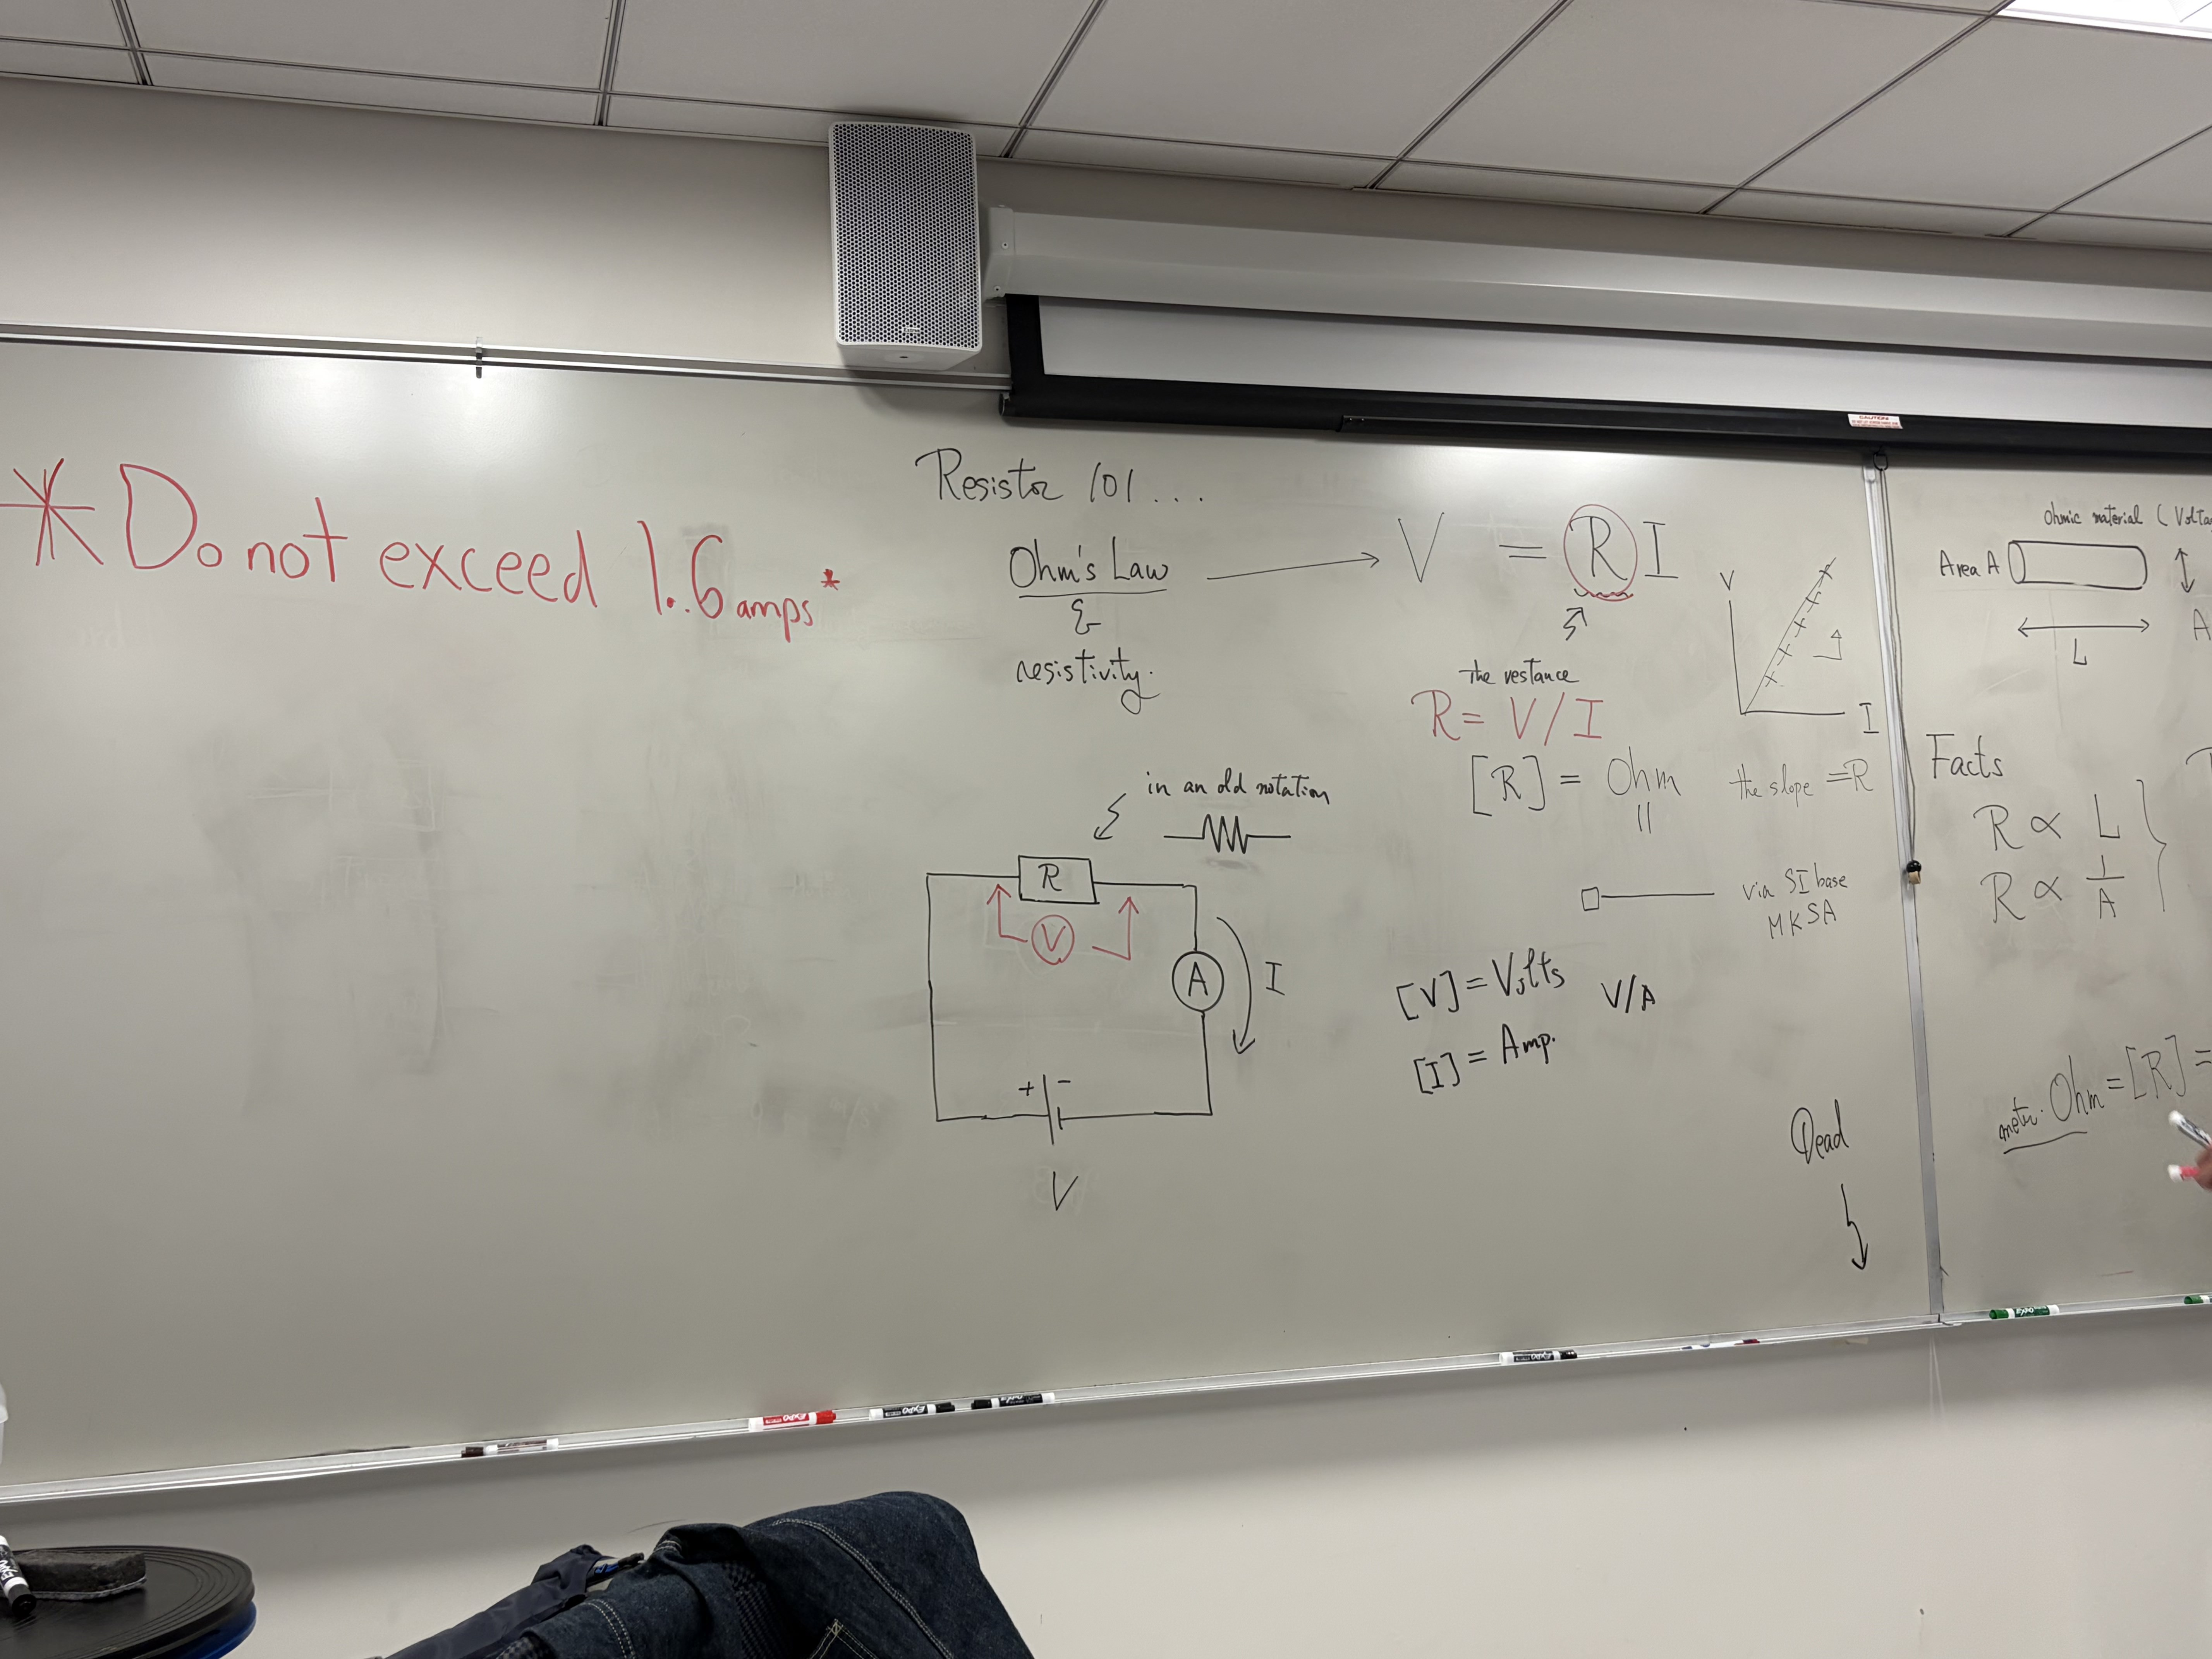
\includegraphics[width=0.92\textwidth]{IMG_3664.jpg}
    \caption{Dr. Ray's whiteboard from the start of lab covering Ohm's Law and the circuit setup.}
\end{figure}

\begin{figure}[H]
    \centering
    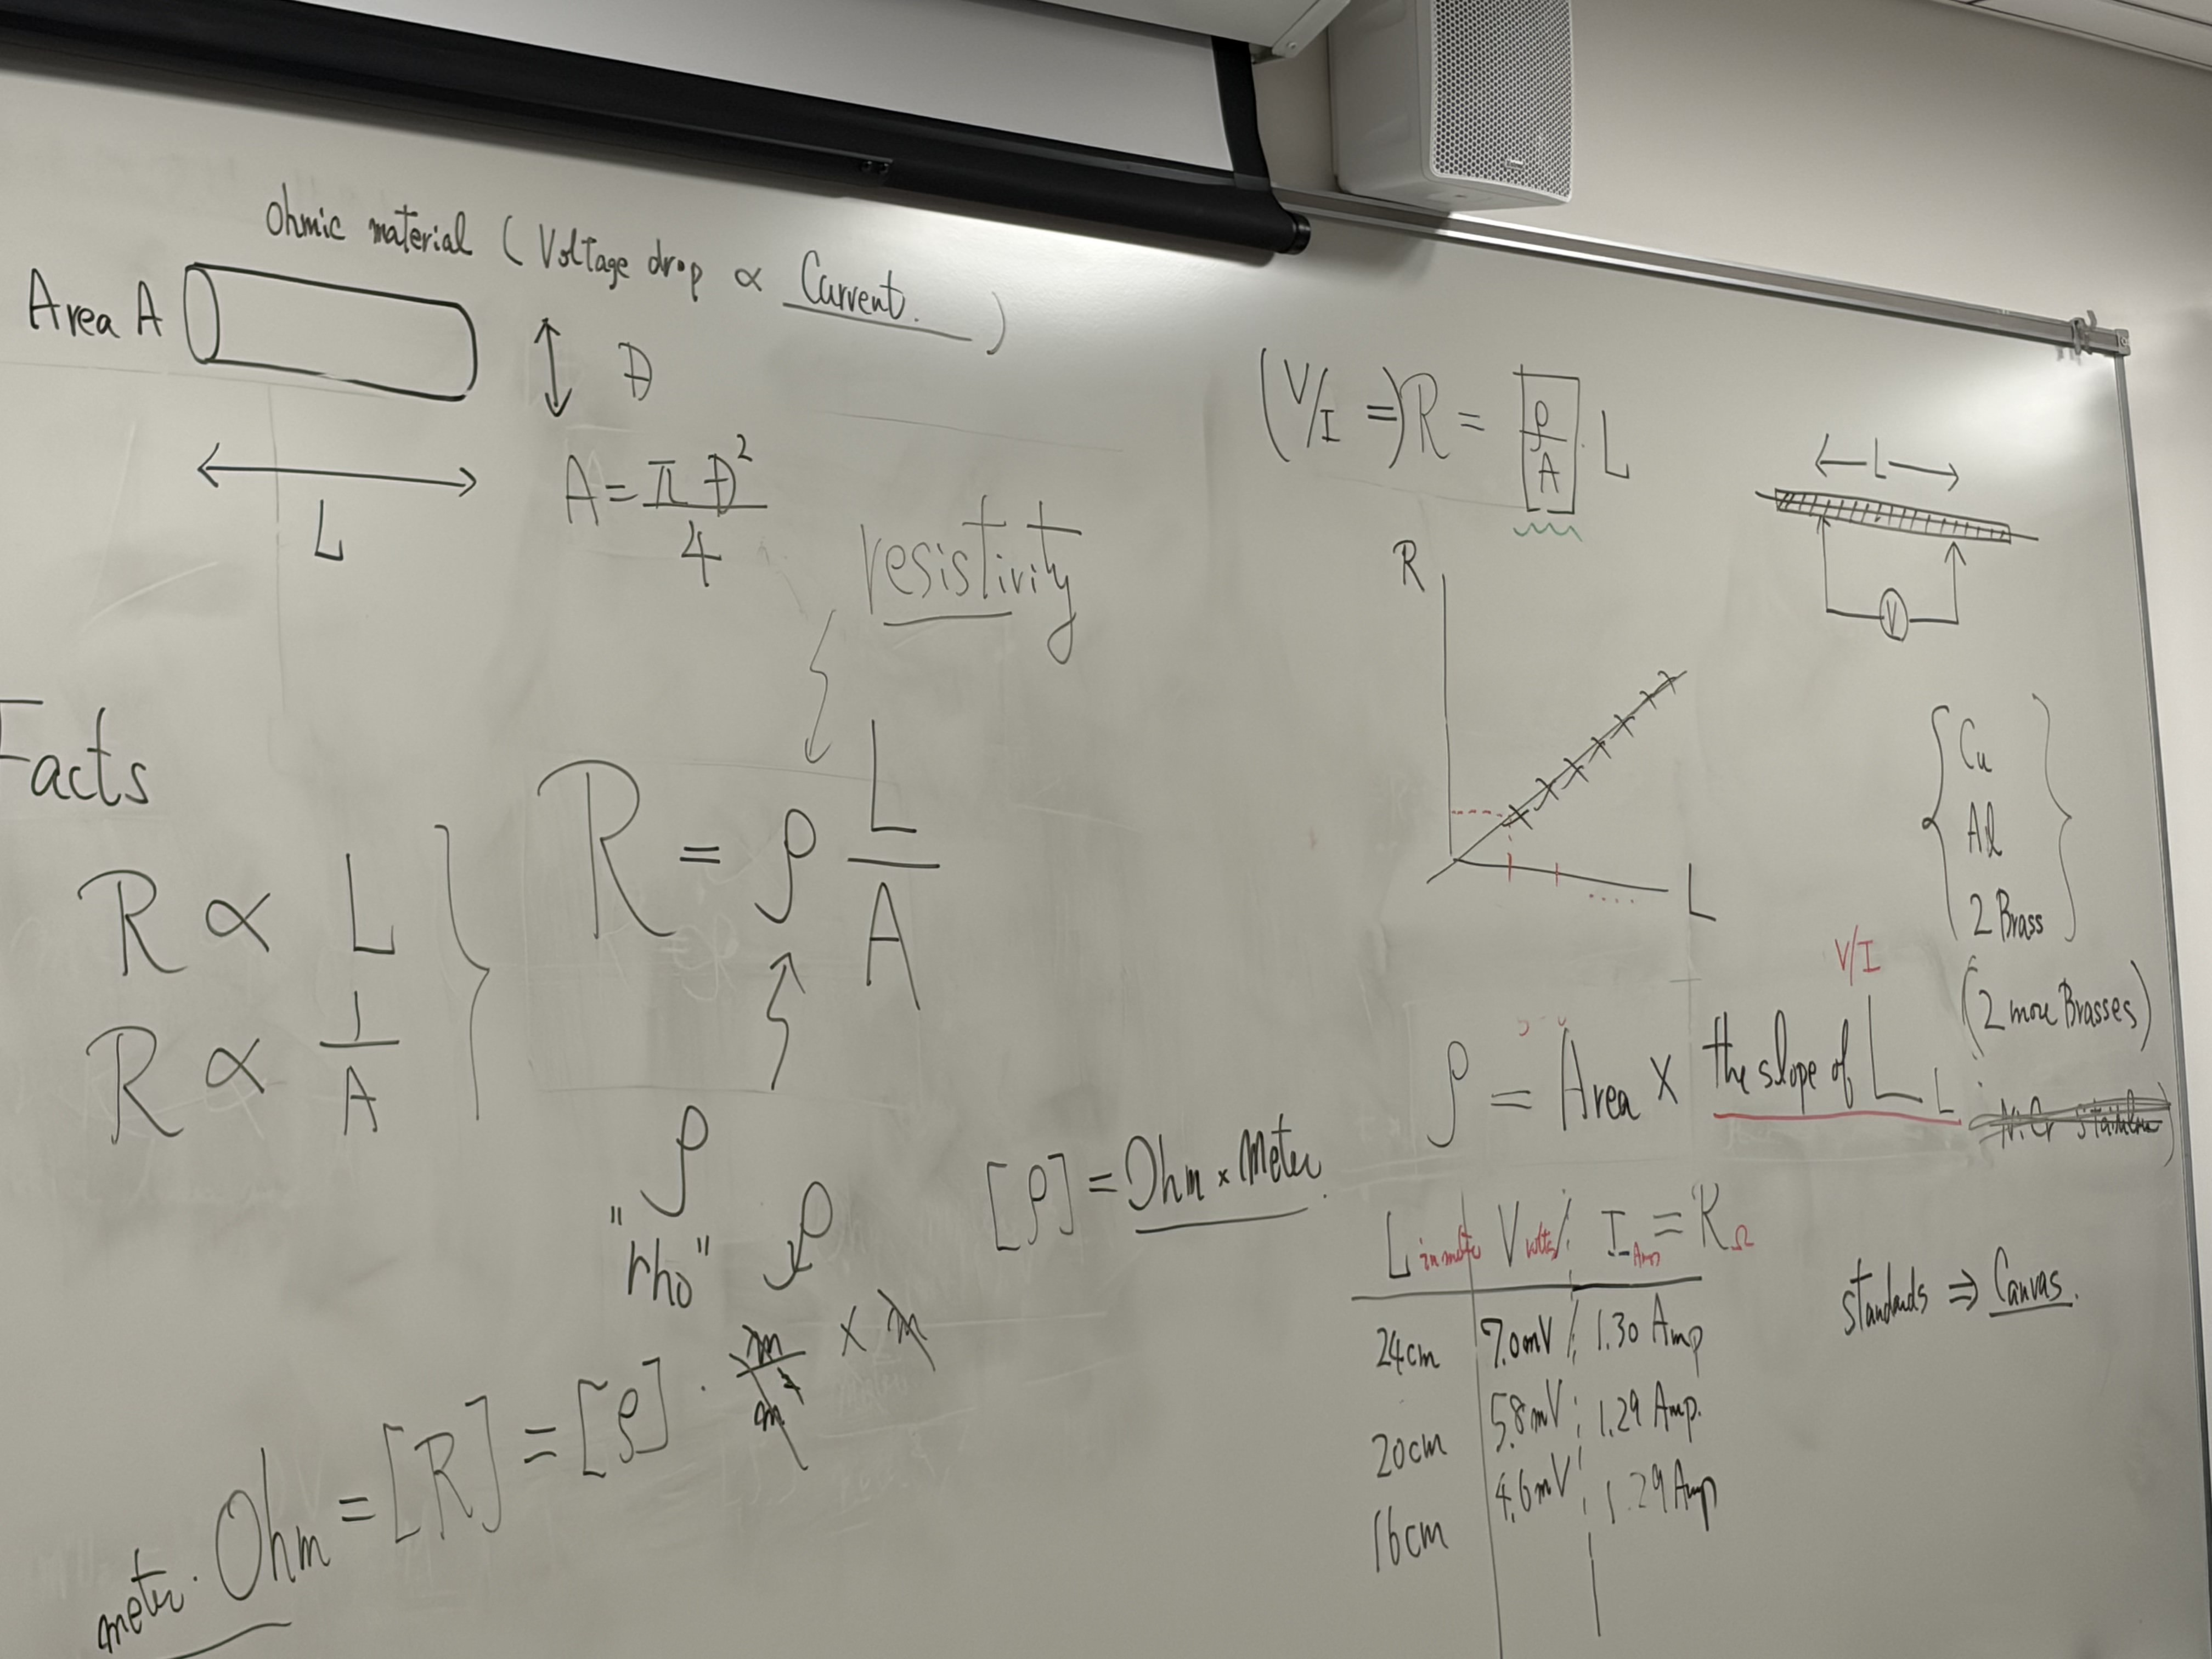
\includegraphics[width=0.92\textwidth]{IMG_3665.jpg}
    \caption{Dr. Ray explaining the resistivity formula $R = \rho L/A$ and how to extract $\rho$ from the slope of an $R$ vs. $L$ graph.}
\end{figure}

\section*{Procedure}

The apparatus passes current through the full wire while a sliding voltmeter probe measures the voltage across a selected section. This keeps the probe contact resistance out of the measurement, which matters because these resistances are very small (milliohm range).

For each wire we kept the reference probe at 0 cm and moved the slider from 14 to 24 cm in 2 cm steps. The four wires tested were:

\begin{itemize}
    \item Copper (Cu) -- 0.040 in (1.016 mm)
    \item Aluminum (Al) -- 0.040 in (1.016 mm)
    \item Brass, thick -- 0.050 in (1.270 mm)
    \item Brass, thin -- 0.032 in (0.813 mm)
\end{itemize}

\section*{Data and Results}

Each table is shown next to its $R$ vs. $L$ graph. The solid line is our measured fit and the dashed line is the expected line based on the manufacturer's standard resistivity value.

% -------------------------------------------------------
% COPPER
% -------------------------------------------------------
\vspace{6pt}
\noindent\rule{\textwidth}{0.4pt}
\vspace{2pt}

\noindent\textbf{Copper} \quad $d = 0.040\ \text{in} = 1.016\ \text{mm}$, \quad $I \approx 1.33\ \text{A}$, \quad $\rho_\text{std} = 1.8 \times 10^{-8}\ \Omega\cdot\text{m}$
\vspace{4pt}

\noindent
\begin{minipage}[c]{0.44\textwidth}
\centering
\captionof{table}{Copper wire measurements (V in mV, converted for $R$).}
\vspace{2pt}
\small
\begin{tabular}{cccc}
\toprule
$L$ (cm) & $V$ (mV) & $I$ (A) & $R$ ($\Omega$) \\
\midrule
24 & 7.2 & 1.32 & 0.00545 \\
22 & 6.2 & 1.31 & 0.00473 \\
20 & 5.7 & 1.34 & 0.00425 \\
18 & 5.3 & 1.32 & 0.00402 \\
16 & 4.8 & 1.35 & 0.00356 \\
14 & 4.2 & 1.33 & 0.00316 \\
\bottomrule
\end{tabular}
\end{minipage}
\hfill
\begin{minipage}[c]{0.53\textwidth}
\centering
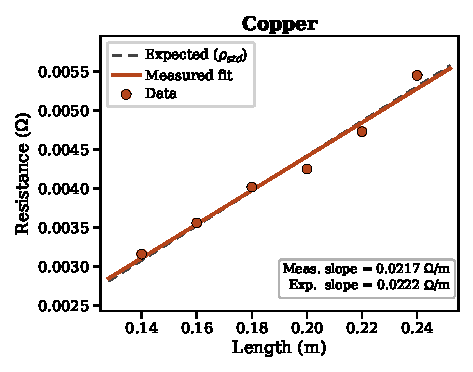
\includegraphics[width=\textwidth]{copper_graph.pdf}
\captionof{figure}{$R$ vs. $L$ for copper. Measured slope $= 0.0217\ \Omega/\text{m}$; expected slope $= 0.0222\ \Omega/\text{m}$.}
\end{minipage}

% -------------------------------------------------------
% BRASS THICK
% -------------------------------------------------------
\vspace{6pt}
\noindent\rule{\textwidth}{0.4pt}
\vspace{2pt}

\noindent\textbf{Brass, Thick} \quad $d = 0.050\ \text{in} = 1.270\ \text{mm}$, \quad $I = 1.27\ \text{A}$, \quad $\rho_\text{std} = 7.0 \times 10^{-8}\ \Omega\cdot\text{m}$
\vspace{4pt}

\noindent
\begin{minipage}[c]{0.44\textwidth}
\centering
\captionof{table}{Thick brass wire measurements (V in volts).}
\vspace{2pt}
\small
\begin{tabular}{cccc}
\toprule
$L$ (cm) & $V$ (V) & $I$ (A) & $R$ ($\Omega$) \\
\midrule
24 & 0.016 & 1.27 & 0.01260 \\
22 & 0.015 & 1.27 & 0.01181 \\
20 & 0.014 & 1.27 & 0.01102 \\
18 & 0.012 & 1.27 & 0.00945 \\
16 & 0.011 & 1.27 & 0.00866 \\
14 & 0.009 & 1.27 & 0.00709 \\
\bottomrule
\end{tabular}
\end{minipage}
\hfill
\begin{minipage}[c]{0.53\textwidth}
\centering
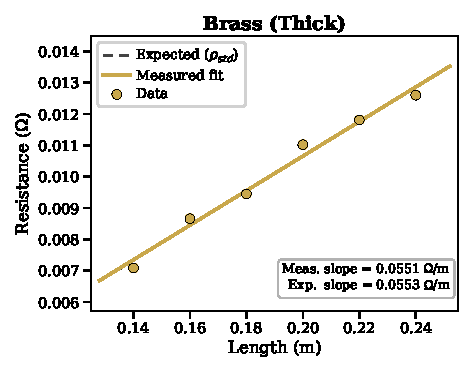
\includegraphics[width=\textwidth]{brass_thick_graph.pdf}
\captionof{figure}{$R$ vs. $L$ for thick brass. Measured slope $= 0.0551\ \Omega/\text{m}$; expected slope $= 0.0553\ \Omega/\text{m}$.}
\end{minipage}

% -------------------------------------------------------
% ALUMINUM
% -------------------------------------------------------
\vspace{6pt}
\noindent\rule{\textwidth}{0.4pt}
\vspace{2pt}

\noindent\textbf{Aluminum} \quad $d = 0.040\ \text{in} = 1.016\ \text{mm}$, \quad $I = 0.92\ \text{A}$, \quad $\rho_\text{std} = 4.9 \times 10^{-8}\ \Omega\cdot\text{m}$
\vspace{4pt}

\noindent
\begin{minipage}[c]{0.44\textwidth}
\centering
\captionof{table}{Aluminum wire measurements (V in mV, converted for $R$).}
\vspace{2pt}
\small
\begin{tabular}{cccc}
\toprule
$L$ (cm) & $V$ (mV) & $I$ (A) & $R$ ($\Omega$) \\
\midrule
24 & 16.1 & 0.92 & 0.01750 \\
22 & 14.8 & 0.92 & 0.01609 \\
20 & 13.4 & 0.92 & 0.01457 \\
18 & 12.1 & 0.92 & 0.01315 \\
16 & 10.7 & 0.92 & 0.01163 \\
\bottomrule
\end{tabular}
\end{minipage}
\hfill
\begin{minipage}[c]{0.53\textwidth}
\centering
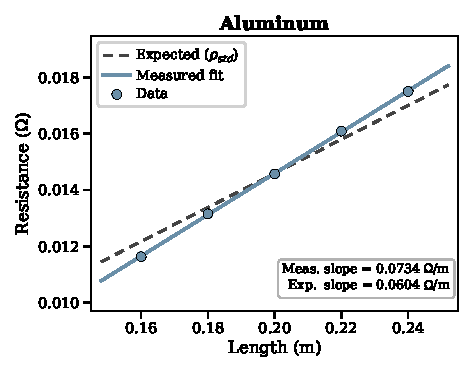
\includegraphics[width=\textwidth]{aluminum_graph.pdf}
\captionof{figure}{$R$ vs. $L$ for aluminum. Measured slope $= 0.0734\ \Omega/\text{m}$; expected slope $= 0.0604\ \Omega/\text{m}$.}
\end{minipage}

% -------------------------------------------------------
% BRASS THIN
% -------------------------------------------------------
\vspace{6pt}
\noindent\rule{\textwidth}{0.4pt}
\vspace{2pt}

\noindent\textbf{Brass, Thin} \quad $d = 0.032\ \text{in} = 0.813\ \text{mm}$, \quad $I = 0.94\ \text{A}$, \quad $\rho_\text{std} = 7.0 \times 10^{-8}\ \Omega\cdot\text{m}$
\vspace{4pt}

\noindent
\begin{minipage}[c]{0.44\textwidth}
\centering
\captionof{table}{Thin brass wire measurements (V in mV, converted for $R$).}
\vspace{2pt}
\small
\begin{tabular}{cccc}
\toprule
$L$ (cm) & $V$ (mV) & $I$ (A) & $R$ ($\Omega$) \\
\midrule
24 & 32.5 & 0.94 & 0.03457 \\
22 & 29.7 & 0.94 & 0.03160 \\
20 & 27.1 & 0.94 & 0.02883 \\
18 & 24.6 & 0.94 & 0.02617 \\
16 & 21.7 & 0.94 & 0.02309 \\
\bottomrule
\end{tabular}
\end{minipage}
\hfill
\begin{minipage}[c]{0.53\textwidth}
\centering
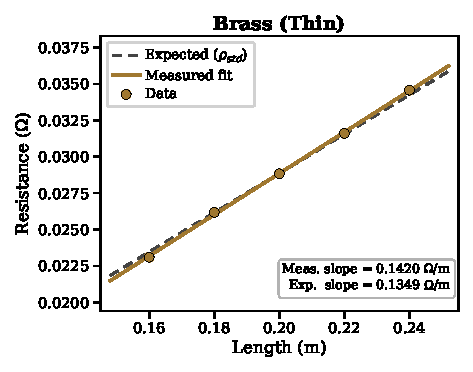
\includegraphics[width=\textwidth]{brass_thin_graph.pdf}
\captionof{figure}{$R$ vs. $L$ for thin brass. Measured slope $= 0.1420\ \Omega/\text{m}$; expected slope $= 0.1349\ \Omega/\text{m}$.}
\end{minipage}

\vspace{6pt}
\noindent\rule{\textwidth}{0.4pt}

\section*{Analysis}

Resistivity is found by rearranging equation~\eqref{eq:resistivity}:
\begin{equation}
    \rho = \text{slope} \times \frac{\pi d^2}{4}
    \label{eq:slope_rho}
\end{equation}

For copper, the regression slope across all six data points was $0.02170\ \Omega/\text{m}$. With $d = 1.016 \times 10^{-3}$ m:
\[
    A = \frac{\pi (1.016 \times 10^{-3})^2}{4} = 8.107 \times 10^{-7}\ \text{m}^2
\]
\[
    \rho_{Cu} = 0.02170 \times 8.107 \times 10^{-7} = 1.759 \times 10^{-8}\ \Omega \cdot \text{m}
\]

The accepted value from the manual is $(1.8 \pm 0.1) \times 10^{-8}\ \Omega \cdot \text{m}$, so our result is well within range:
\[
    \% \ \text{difference} = \frac{|1.759 - 1.8|}{1.8} \times 100\% \approx 2.3\%
\]

Comparing all four wires at 20 cm shows the effect of both material and geometry:

\begin{table}[H]
\centering
\caption{Resistance at 20 cm for all four wires.}
\begin{tabular}{lccc}
\toprule
Material & Diameter (in) & $R$ at 20 cm ($\Omega$) & $\rho_\text{std}$ ($\mu\Omega \cdot \text{cm}$) \\
\midrule
Copper        & 0.040 & 0.00425 & $1.8 \pm 0.1$ \\
Brass (thick) & 0.050 & 0.01102 & $7.0 \pm 0.5$ \\
Aluminum      & 0.040 & 0.01457 & $4.9 \pm 0.1$ \\
Brass (thin)  & 0.032 & 0.02883 & $7.0 \pm 0.5$ \\
\bottomrule
\end{tabular}
\end{table}

Copper had the lowest resistance by far. The two brass wires are the same material but the thin one has about 2.44 times the resistance of the thick one, which matches the expected area ratio of $(0.050/0.032)^2 \approx 2.44$.

\section*{Discussion}

Overall the results matched the expected values well. Copper and thick brass were very close to their standard slopes. Aluminum was a bit higher than expected, and the thin brass was slightly off, which may be due to small variations in the actual wire diameter.

The main source of error was the voltage readings, especially for copper where values were only a few millivolts. Small fluctuations in current or probe placement at those levels can noticeably affect the result.

\section*{Conclusion}

We measured the resistivity of copper, aluminum, and two brass wires. Our copper result of $1.76 \times 10^{-8}\ \Omega \cdot \text{m}$ was within 2.3\% of the accepted value. All four wires showed resistance increasing linearly with length, and the two brass wires confirmed that a thinner wire has higher resistance at the same length, as predicted by $R = \rho L/A$.

\end{document}